\section{Motivation and Scope}

There has been a strong desire for a more space- and/or runtime-efficient
representation for \code{map} among C++ users for some time now.  This has
motivated discussions among the members of SG14 resulting in a
paper\footnote{See P0038R0,
  \href{http://www.open-std.org/jtc1/sc22/wg21/docs/papers/2015/p0038r0.html}{here}.},
numerous articles and talks, and an implementation in Boost,
\code{boost::container::flat_map}\footnote{Part of Boost.Container,
  \href{http://www.boost.org/doc/libs/1_61_0/doc/html/container.html}{here}.}.
Virtually everyone who makes games, embedded, or system software in C++ uses
the Boost implementation or one that they rolled themselves.\\

Here are some numbers that show why.  The graphs that follow show runtimes for
different \code{map}-like associative containers.  The containers used are
Boost.FlatMap, \code{map}, and two thin wrappers over a sorted \code{vector};
the ``custom pair'' version of the sorted \code{vector} uses a simple
\code{struct} instead of \code{pair} for its value type.  All containers use
an \code{int} as the key type and an \code{int} or a \code{struct} with 5
\code{double}s for the value type.\\

All the graphs below were produced on Windows with MSVC 2015.  Similar results
were obtained on Linux, with Clang 3.9 and libc++, and with g++ 4.8.4 and
libstdc++.\\

These first four graphs cover the \code{int}-value-type case.  The first graph
shows insertion of N elements with random keys; the second shows full
iteration across all N elements; the third shows \code{map.lower_bound()}
called once for each key used in the original insertions; and the fourth shows
erasure of all N elements, by the keys used in the original insertions.

\begin{center}
    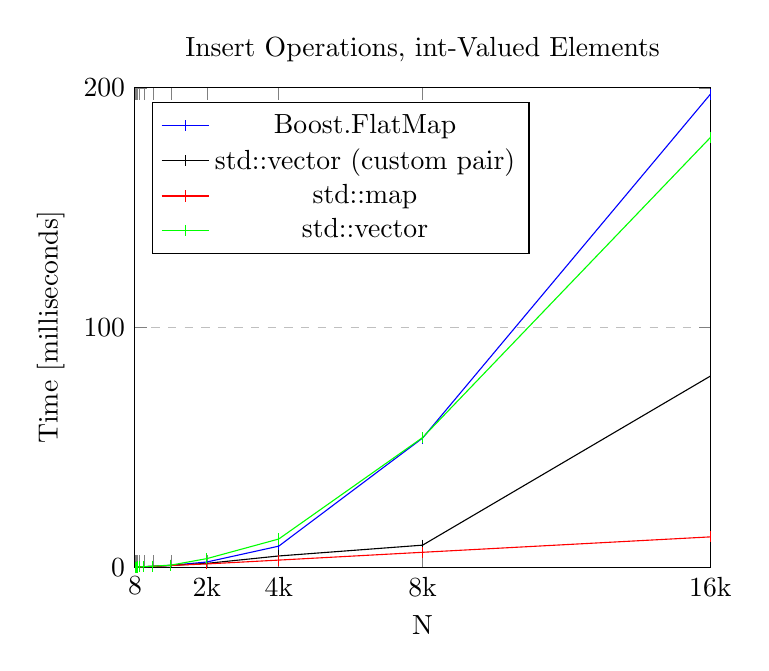
\begin{tikzpicture}
    \begin{axis}[
        width=3.5in,
        title={Insert Operations, int-Valued Elements},
        xlabel={N},
        ylabel={Time [milliseconds]},
        xmin=0, xmax=16384,
        ymin=0, ymax=200.0,
        xtick={8,16,32,64,128,256,512,1024,2048,4096,8192,16384,32768},
        xticklabels={8,,,,,,,,2k,4k,8k,16k,32k},
        ytick={0.0,100.0,200.0,300.0},
        legend pos=north west,
        ymajorgrids=true,
        grid style=dashed,
        scaled x ticks=false,
        scaled y ticks=true,
        legend entries={Boost.FlatMap,std::vector (custom pair),std::map,std::vector},
        ]

    \addplot[color=blue,mark=|,]
        coordinates {(8,0.0057276)(16,0.0107692)(32,0.0214416)(64,0.0445022)(128,0.075722)(256,0.16104)(512,0.334246)(1024,0.735082)(2048,2.12155)(4096,8.74114)(8192,53.8606)(16384,197.326)};

    \addplot[color=black,mark=|,]
        coordinates {(8,0.0054478)(16,0.0105188)(32,0.0206046)(64,0.0422692)(128,0.079827)(256,0.150927)(512,0.300043)(1024,0.668588)(2048,1.55036)(4096,4.64456)(8192,9.15801)(16384,79.7067)};

    \addplot[color=red,mark=|,]
        coordinates {(8,0.0058806)(16,0.011215)(32,0.0223082)(64,0.0439032)(128,0.0759592)(256,0.164184)(512,0.304031)(1024,0.700694)(2048,1.31409)(4096,2.92277)(8192,6.18145)(16384,12.6075)};

    \addplot[color=green,mark=|,]
        coordinates {(8,0.0054478)(16,0.0106014)(32,0.020604)(64,0.0427862)(128,0.081883)(256,0.176755)(512,0.381274)(1024,0.825943)(2048,3.53353)(4096,11.7211)(8192,54.0627)(16384,179.264)};

    \end{axis}
\end{tikzpicture}
\end{center}


As one might expect, insertionion takes longer in contiguous-storage
implementations.  Boost.FlatMap and a sorted \code{vector<pair<int, int>>}
have superlinear growth in insertion time.  While the curve for sorted
\code{vector} using a custom \code{struct} instead of a \code{pair} is
superlinear as well, it is dramatically flatter in its growth -- much closer
to node-based \code{map}.

\begin{center}
    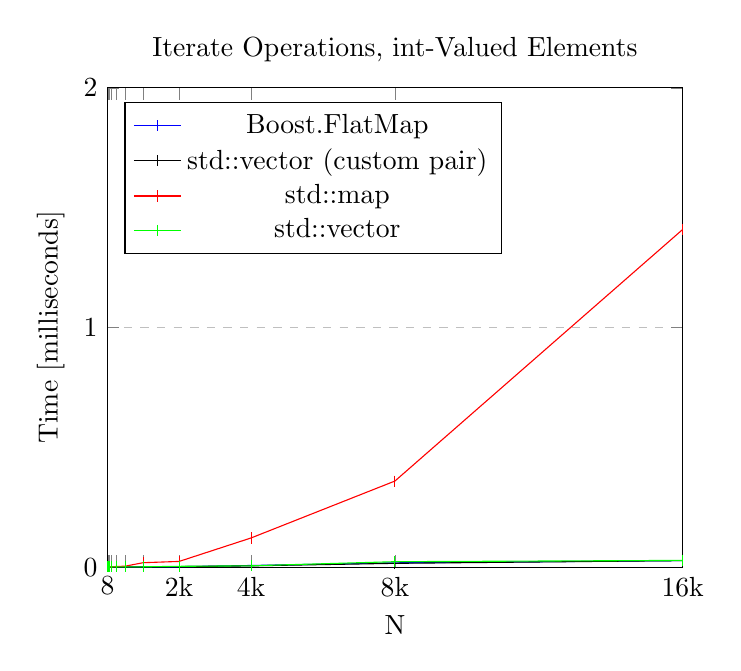
\begin{tikzpicture}
    \begin{axis}[
        width=3.5in,
        title={Iterate Operations, int-Valued Elements},
        xlabel={N},
        ylabel={Time [milliseconds]},
        xmin=0, xmax=16384,
        ymin=0, ymax=2.0,
        xtick={8,16,32,64,128,256,512,1024,2048,4096,8192,16384,32768},
        xticklabels={8,,,,,,,,2k,4k,8k,16k,32k},
        ytick={0.0,1.0,2.0,3.0},
        legend pos=north west,
        ymajorgrids=true,
        grid style=dashed,
        scaled x ticks=false,
        scaled y ticks=true,
        legend entries={Boost.FlatMap,std::vector (custom pair),std::map,std::vector},
        ]

    \addplot[color=blue,mark=|,]
        coordinates {(8,0.000615)(16,0.0007266)(32,0.0006982)(64,0.0006702)(128,0.0006286)(256,0.00088)(512,0.0008798)(1024,0.0009358)(2048,0.0016902)(4096,0.006691)(8192,0.0177678)(16384,0.0270706)};

    \addplot[color=black,mark=|,]
        coordinates {(8,0.0006704)(16,0.0007122)(32,0.000628)(64,0.0010894)(128,0.0006288)(256,0.0007542)(512,0.0007128)(1024,0.0010618)(2048,0.0019976)(4096,0.0052664)(8192,0.0157284)(16384,0.027182)};

    \addplot[color=red,mark=|,]
        coordinates {(8,0.0007266)(16,0.0007544)(32,0.0009082)(64,0.0013968)(128,0.001271)(256,0.0024584)(512,0.0038694)(1024,0.0183544)(2048,0.0236622)(4096,0.12158)(8192,0.359138)(16384,1.40895)};

    \addplot[color=green,mark=|,]
        coordinates {(8,0.0007126)(16,0.0006844)(32,0.000629)(64,0.000726)(128,0.0005868)(256,0.0008658)(512,0.000866)(1024,0.0011592)(2048,0.0032544)(4096,0.005392)(8192,0.0225308)(16384,0.0279502)};

    \end{axis}
\end{tikzpicture}
\end{center}


For all variants but \code{map}, iteration is relatively similar, and much
faster that \code{map}'s.

\begin{center}
    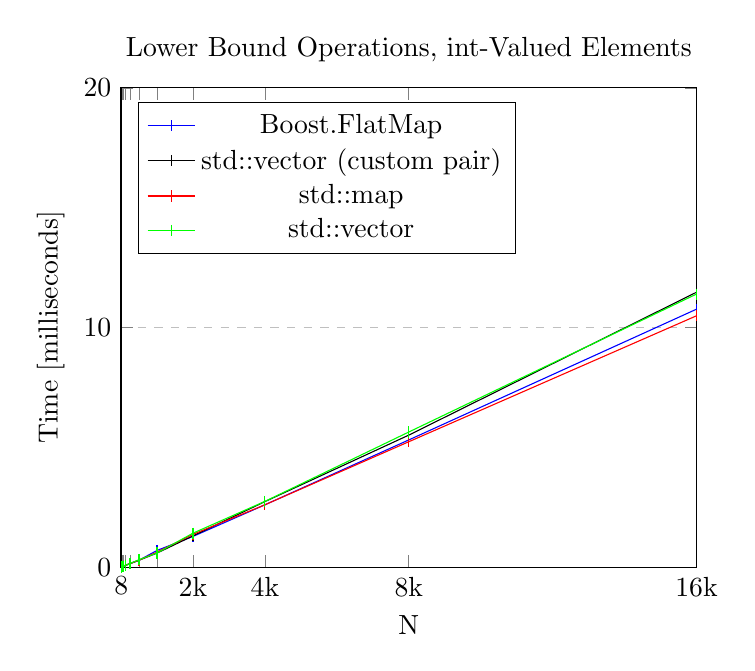
\begin{tikzpicture}
    \begin{axis}[
        width=3.5in,
        title={Lower Bound Operations, int-Valued Elements},
        xlabel={N},
        ylabel={Time [milliseconds]},
        xmin=0, xmax=16384,
        ymin=0, ymax=20.0,
        xtick={8,16,32,64,128,256,512,1024,2048,4096,8192,16384,32768},
        xticklabels={8,,,,,,,,2k,4k,8k,16k,32k},
        ytick={0.0,10.0,20.0,30.0},
        legend pos=north west,
        ymajorgrids=true,
        grid style=dashed,
        scaled x ticks=false,
        scaled y ticks=true,
        legend entries={Boost.FlatMap,std::vector (custom pair),std::map,std::vector},
        ]

    \addplot[color=blue,mark=|,]
        coordinates {(8,0.0048888)(16,0.0097784)(32,0.0194572)(64,0.0387614)(128,0.0719788)(256,0.15062)(512,0.28597)(1024,0.694518)(2048,1.28027)(4096,2.59875)(8192,5.30652)(16384,10.7638)};

    \addplot[color=black,mark=|,]
        coordinates {(8,0.0050988)(16,0.0099448)(32,0.0195278)(64,0.0388038)(128,0.07649)(256,0.143357)(512,0.283663)(1024,0.585327)(2048,1.30256)(4096,2.73305)(8192,5.50775)(16384,11.4704)};

    \addplot[color=red,mark=|,]
        coordinates {(8,0.0050146)(16,0.0098338)(32,0.0192202)(64,0.0385802)(128,0.0713516)(256,0.147967)(512,0.291103)(1024,0.62142)(2048,1.36704)(4096,2.59982)(8192,5.2311)(16384,10.4881)};

    \addplot[color=green,mark=|,]
        coordinates {(8,0.0051684)(16,0.0099876)(32,0.0194584)(64,0.0389582)(128,0.071921)(256,0.14913)(512,0.306088)(1024,0.587018)(2048,1.41528)(4096,2.74166)(8192,5.63672)(16384,11.3943)};

    \end{axis}
\end{tikzpicture}
\end{center}


\code{lower_bound()} performance is roughly similar across all the
implementations, and they all show superlinear growth.  Note that
Boost.FlatMap performs the best here.

\begin{center}
    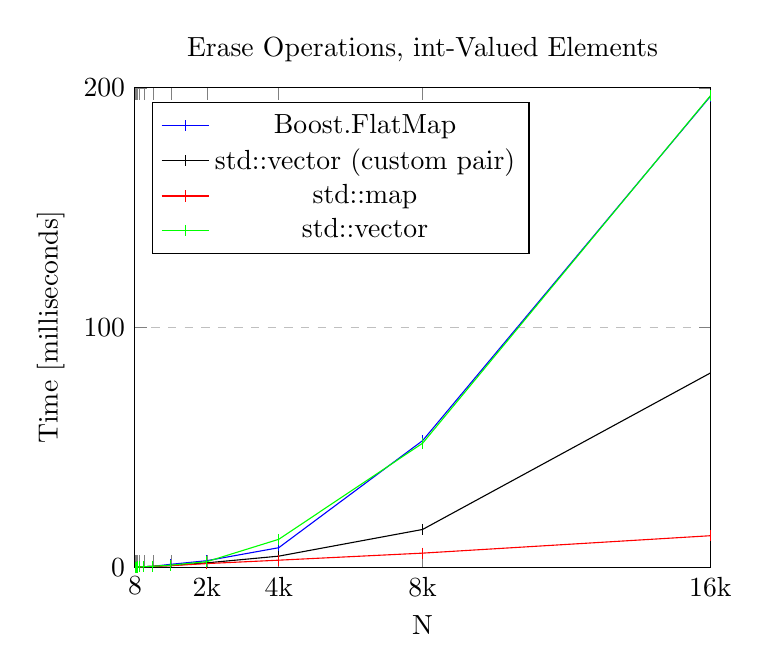
\begin{tikzpicture}
    \begin{axis}[
        width=3.5in,
        title={Erase Operations, int-Valued Elements},
        xlabel={N},
        ylabel={Time [milliseconds]},
        xmin=0, xmax=16384,
        ymin=0, ymax=200.0,
        xtick={8,16,32,64,128,256,512,1024,2048,4096,8192,16384,32768},
        xticklabels={8,,,,,,,,2k,4k,8k,16k,32k},
        ytick={0.0,100.0,200.0,300.0},
        legend pos=north west,
        ymajorgrids=true,
        grid style=dashed,
        scaled x ticks=false,
        scaled y ticks=true,
        legend entries={Boost.FlatMap,std::vector (custom pair),std::map,std::vector},
        ]

    \addplot[color=blue,mark=|,]
        coordinates {(8,0.0051958)(16,0.010211)(32,0.020157)(64,0.040955)(128,0.0754832)(256,0.170906)(512,0.325072)(1024,1.15706)(2048,2.66907)(4096,8.09283)(8192,52.7669)(16384,196.443)};

    \addplot[color=black,mark=|,]
        coordinates {(8,0.0056156)(16,0.0100154)(32,0.0197504)(64,0.0371264)(128,0.072537)(256,0.146989)(512,0.296743)(1024,0.660295)(2048,1.7662)(4096,4.56922)(8192,15.7069)(16384,80.9934)};

    \addplot[color=red,mark=|,]
        coordinates {(8,0.0054056)(16,0.0106724)(32,0.021665)(64,0.0408292)(128,0.0730398)(256,0.156864)(512,0.321395)(1024,0.600078)(2048,1.46327)(4096,2.88768)(8192,5.82895)(16384,13.094)};

    \addplot[color=green,mark=|,]
        coordinates {(8,0.005336)(16,0.0100574)(32,0.0200302)(64,0.0406328)(128,0.0744786)(256,0.16494)(512,0.336185)(1024,0.813833)(2048,2.27156)(4096,11.5982)(8192,51.69)(16384,196.705)};

    \end{axis}
\end{tikzpicture}
\end{center}


Erasure has a similar performance profile to insertion, except that the sorted
\code{vector<pair<int, int>>} performs substantially better than
Boost.FlatMap.\\


\subsection{Implications}

TODO Iteration is vastly cheaper for contiguous-storage variants.  It has been
suggested that a \code{map} with a custom allocator can achieve similar
performance to flat data structures, but this would not apply to iteration
performance, unless the values were added to the \code{map} in sorted order.\\

In all the graphs above, the reason the custom-\code{pair} sorted vector
performs so much better than \code{vector<pair<int, int>>} seems to be that
the custom-\code{pair} type has \code{nothrow} special functions.
Implementing all the special functions and adding \code{nothrow(false)} to
each makes the custom-\code{pair} version perform identically to the
\code{pair<int, int>} version.

Boost.FlatMap differs quite a bit from a sorted \code{vector}.  Clearly there
are a lot of QOI choices to make in implementing a standard \code{flat_map}.
